\documentclass[]{article}
% ========== 基础宏包 ==========
\usepackage{algorithm}
\usepackage{authblk} 
\usepackage{verbatim}
\usepackage{algpseudocode}
\usepackage{float}
\usepackage{lipsum}
\usepackage{amsmath}
\usepackage{color}
\usepackage{appendix}
\usepackage{soul}
\usepackage{amsthm,amsmath,multirow,amssymb}
\usepackage{mathrsfs} 
\usepackage{algorithmicx}
\usepackage{pgfplots} 
\pgfplotsset{compat=1.18} 
\usepackage{tikz} 
\usepackage[utf8]{inputenc}
\usepackage[T1]{fontenc}

\usepackage{booktabs,tabularx,bigstrut}
\usepackage{threeparttable}
\usepackage{epstopdf}
\usepackage{xcolor}

\usepackage{array}
\usepackage{makecell}
\usepackage{adjustbox}
\usepackage{graphicx} 
\usepackage{longtable}

\usepackage{url} 
\usepackage{enumitem} 
\usepackage{subcaption} 

% ========== 设置宏包选项 ==========
\usepackage[british]{babel}
\usepackage{mdwlist}

\usepackage[doublespacing]{setspace}% To produce a `double spaced' document if required
\setlength\parindent{24pt}% To increase paragraph indentation when line spacing is doubled

% ========== 参考文献设置 ==========
\usepackage[authoryear,sort]{natbib}% Citation support using natbib.sty
\bibpunct[, ]{(}{)}{;}{a}{,}{,}% Citation support using natbib.sty
\renewcommand\bibfont{\fontsize{10}{12}\selectfont}% To set the list of references in 10 point font using natbib.sty

% ========== 算法格式重定义 ==========
\renewcommand{\algorithmicrequire}{\textbf{Input:}}  % Use Input in the format of Algorithm
\renewcommand{\algorithmicensure}{\textbf{Output:}} % Use Output in the format of Algorithm

% ========== 定理环境 ==========
\theoremstyle{plain}% Theorem-like structures provided by amsthm.sty
\newtheorem{theorem}{Theorem}[section]
\newtheorem{lemma}[theorem]{Lemma}
\newtheorem{corollary}[theorem]{Corollary}
\newtheorem{proposition}[theorem]{Proposition}
\newtheorem{claim}{Claim}
\newtheorem{problem}{Problem}
\newtheorem{property}{Property}

\theoremstyle{definition}
\newtheorem{definition}[theorem]{Definition}
\newtheorem{example}[theorem]{Example}

\theoremstyle{remark}
\newtheorem{remark}{Remark}
\newtheorem{notation}{Notation}

% ========== 数学命令定义 ==========
\def\be{\begin{equation}}
\def\ee{\end{equation}}
\def\ba{\begin{array}}
\def\ea{\end{array}}

\usepackage{threeparttable} 

\def\UrlBreaks{\do\A\do\B\do\C\do\D\do\E\do\F\do\G\do\H\do\I\do\J
\do\K\do\L\do\M\do\N\do\O\do\P\do\Q\do\R\do\S\do\T\do\U\do\V
\do\W\do\X\do\Y\do\Z\do\[\do\\\do\]\do\^\do\_\do\`\do\a\do\b
\do\c\do\d\do\e\do\f\do\g\do\h\do\i\do\j\do\k\do\l\do\m\do\n
\do\o\do\p\do\q\do\r\do\s\do\t\do\u\do\v\do\w\do\x\do\y\do\z
\do\.\do\@\do\\\do\/\do\!\do\_\do\|\do\;\do\>\do\]\do\)\do\,
\do\?\do\'\do+\do\=\do\#}
\theoremstyle{plain}% Theorem-like structures provided by amsthm.sty
\algdef{SE}[DOWHILE]{Do}{doWhile}{\algorithmicdo}[1]{\algorithmicwhile\ #1}%

\newcounter{bean}
\newcommand{\RE}{\mathbb{R}}

% ========== 页面设置 ==========
\setlength{\oddsidemargin}{-0.1in}
\setlength{\evensidemargin}{0.25in} \setlength{\textwidth}{6.5in}
\setlength{\topmargin}{-0.3in} \setlength{\textheight}{8.5in}
\pagenumbering{arabic}
\parskip 1.75\parskip plus 3pt minus 1pt
\renewcommand{\baselinestretch}{1.0}
\newcommand{\PSbox}[3]{\mbox{\rule{0in}{#3}\special{psfile=#1}\hspace{#2}}}
\newcommand{\beqn}{\begin{eqnarray}}
\newcommand {\eeqn}{\end{eqnarray}}

% ========== 数学符号定义 ==========
\def\ov{\overline}
\def\remark{\noindent{\bf Remark}:\ }
\def\proof{\noindent{\bf Proof}:\ }
\def\QED{\hfill{$\rule{6pt}{6pt}$} \newline}
%\def\qed{\hfill{$\rule{6pt}{6pt}$} \newline}
\def\qed{\hspace*{10pt}\hfill{$\square$}\hfilneg\par}
\def\square{\mathchoice\sqr54\sqr54\sqr{2.1}3\sqr{1.5}3}
\def\sqr#1#2{{\vcenter{\hrule height .#2pt
      \hbox{\vrule width .#2pt height#1pt \kern#1pt\vrule width.#2pt}
      \hrule height.#2pt}}}

\def\half{\frac{1}{2}}
\newcommand{\remove}[1]{}
\def\text{}
\def\SUM{\displaystyle\sum}
\def\PROD{\displaystyle\prod}
\newcommand{\W}{{\mathcal W}}
\newcommand{\R}{{\mathcal R}}
\renewcommand\baselinestretch{1.5}
\newcommand{\tabincell}[2]{\begin{tabular}{@{}#1@{}}#2\end{tabular}}
\def\half{\frac{1}{2}}
\setlength{\belowcaptionskip}{10pt}

% ========== 可断页算法环境 ==========
\makeatletter
\newenvironment{breakablealgorithm}
  {\begin{center}
     \refstepcounter{algorithm}
     \hrule height.8pt depth0pt \kern2pt
     \renewcommand{\caption}[2][\relax]{%
       {\raggedright\textbf{\ALG@name~\thealgorithm} ##2\par}%
       \ifx\relax##1\relax
         \addcontentsline{loa}{algorithm}{\protect\numberline{\thealgorithm}##2}%
       \else
         \addcontentsline{loa}{algorithm}{\protect\numberline{\thealgorithm}##1}%
       \fi
       \kern2pt\hrule\kern2pt
     }
  }
  {\kern2pt\hrule\relax
   \end{center}
  }
\makeatother
    

\begin{document}

\title{\bf When Carbon Meets Capital: Optimizing Supply Chain Network Design with Technology Investment under Cap-and-Trade Policy}
\author[]{}

%\author[1]{Yi Ding}
%\author[1]{Zeyu Pei\thanks{Corresponding author: Zeyu Pei, pei\_zeyu@seu.edu.cn}}
%\author[1]{Tiantian Zeng}

%\affil[1]{Department of Management Science and Engineering, School of Economics and Management, Southeast University, \#2 Sipailou, Nanjing, Jiangsu, 210096, P.R. China}


\date{\today}
    
\maketitle
    
\begin{abstract}
Under the prevailing cap-and-trade policy, enterprises face the dual challenge of profit maximization and carbon emission reduction in supply chain network design (SCND). This study investigates the strategic optimization of a supply chain network under cap-and-trade policy, integrating investment in emission reduction technology. We develop a comprehensive Cap-and-Trade Supply Chain Network Design (CAT-SCND) model that holistically considers carbon emissions from facility establishment, inventory holding, and transportation. The model simultaneously optimizes decisions on facility location, inventory management, pricing, carbon trading, and emission reduction technology investment, formulated as a challenging nonlinear mixed-integer programming problem. To tackle this complexity, we propose a novel hybrid algorithm that combines the global search capability of a genetic algorithm with the precision of a branch-and-price method. Numerical experiments demonstrate that strategically investing in emission reduction technologies can create a win-win outcome, simultaneously increasing corporate profits by an average of 5.12\% and reducing carbon emissions by 27.63\% compared to the non-investment scenario. Furthermore, the emission reduction investment cost coefficient ($\delta$) is identified as a critical factor influencing corporate decisions. These findings provide valuable insights for enterprises seeking to balance economic and environmental objectives and for policymakers aiming to design effective carbon regulations
\end{abstract}
    
    \noindent{\bf Keywords:} Cap-and-trade policy, Supply chain network design, Emission reduction technology investment, Location-inventory-pricing model.
    
    \section{Introduction}
The urgency of climate change has propelled the global adoption of carbon emission policies, 
with cap-and-trade policy emerging as a prominent market-based mechanism. According to the World Bank's State and Trends of Carbon Pricing 2025 \citep{worldbank2025carbon}, 80 carbon pricing instruments are operational globally, covering nearly a quarter of global greenhouse gas emissions. Supply chains are critical to these efforts, as they account for over half of global carbon emissions across sectors such as food, construction, fashion, and logistics \citep{weforum2021netzero}. Consequently, low-carbon supply chain management has become imperative for enterprises seeking to balance economic and environmental objectives.

While the literature on low-carbon supply chain management has expanded significantly, existing studies often address optimization decisions in isolation. Research streams have separately examined location-inventory problems \citep{shen2003joint}, profit-oriented supply chain network design with pricing decisions \citep{shen2006profit}, carbon-constrained operations under cap-and-trade policy \citep{benjaafar2013carbon}, and investment in emission reduction technology \citep{toptal2014joint}. However, these critical decisions—facility location, inventory management, product pricing, carbon trading, and technology investment—are inherently interdependent in practice. For instance, the optimal scale of emission reduction technology investment depends on operational decisions regarding facility locations and inventory levels, which in turn are influenced by product pricing strategies and carbon market dynamics.

This study bridges this research gap by developing an integrated decision-making framework that simultaneously optimizes these interconnected decisions within a unified model under cap-and-trade regulation. As visually summarized in Table \ref{tab:lit_review_summary} of the subsequent literature review, while prior studies have addressed subsets of these decisions (e.g., location-inventory, or inventory-technology investment), none has holistically combined all four critical dimensions: facility location, inventory management, pricing, and emission reduction technology investment under cap-and-trade policy. We formulate the Cap-and-Trade Supply Chain Network Design (CAT-SCND) problem as a nonlinear mixed-integer programming model that captures carbon emissions from facility establishment, inventory holding, and transportation activities. The model enables firms to strategically invest in emission reduction technologies while determining optimal locations for distribution centers, inventory policies, product prices, and carbon trading strategies.

Our main contributions are threefold. First, we develop a novel integrated optimization model that holistically combines location, inventory, pricing, carbon trading, and technology investment decisions under cap-and-trade—a combination not previously addressed in the literature. Second, we propose an efficient hybrid solution methodology that combines genetic algorithms with branch-and-price techniques to solve this complex optimization problem. Third, through extensive numerical experiments, we provide quantitative insights into the economic and environmental benefits of emission reduction technology investment, demonstrating how strategic investments can create win-win outcomes for firms operating under carbon constraints.

The remainder of this paper is organized as follows. Section 2 reviews relevant literature and positions our contribution. Section 3 presents the mathematical formulation of the CAT-SCND model. Section 4 details the hybrid genetic algorithm with branch-and-price solution approach. Section 5 reports numerical experiments and managerial insights. Section 6 concludes with implications and future research directions.

\section{Literature Review}

\subsection{Traditional Location-Inventory Problems}
Facility location and inventory management are two critical, interconnected decisions in supply chain network design (SCND). Early research often treated them separately. The seminal work of \cite{eppen1979effects} demonstrated that demand aggregation at distribution centers (DCs) leverages risk pooling to save inventory costs, spurring integrated location-inventory models. \cite{barahona1998plant} pioneered this integration by combining the EOQ model with facility location, solved via Dantzig-Wolfe decomposition. Subsequent research refined this foundation. \cite{daskin2002inventory} and \cite{shen2003joint} advanced the model by incorporating ordering and safety stock costs, formulating it as a nonlinear integer program. \cite{shen2003joint} reformulated it as a set covering problem and developed an efficient branch-and-price algorithm, proving submodularity in the pricing subproblem under Poisson demand. Later work focused on algorithmic improvements and practical extensions. \cite{shu2005stochastic} and \cite{shu2011market} designed more general algorithms for the pricing subproblem, while others introduced capacity constraints \cite{ozsen2008capacitated}, demand splitting \cite{ozsen2009facility}, multi-commodity flows \cite{wu2014computational}, and third-party logistics \cite{wang2022joint}. This paper builds upon the single-echelon location-inventory framework, extending it with pricing and carbon policy considerations.

\subsection{Profit-Maximizing Supply Chain Network Design}
Research on profit-maximizing SCND, where firms use pricing to selectively serve markets, is less extensive. Early studies like \cite{zhang2001profit} and \cite{geunes2004economic} focused on standalone location or inventory models with demand selection. A significant integration was achieved by \cite{shen2006profit}, who proposed a profit-maximizing model that simultaneously decides DC locations, retailer assignments, inventory policies, and product prices under deterministic demand, solved via branch-and-price. This work has been extended in several directions: \cite{shu2012logistics} considered a multi-echelon inventory context, \cite{ahmadi2015incorporating} studied multi-commodity scenarios with price-sensitive demand, and \cite{li2019capacitated} incorporated capacity constraints. Our model extends this profit-oriented tradition by embedding it within a carbon-regulated environment.

\subsection{Supply Chain Network Design under Cap-and-Trade Policy}
The adoption of carbon policies has made low-carbon SCND imperative. Cap-and-trade, a market-based mechanism, has received significant attention. Foundational work by \cite{benjaafar2013carbon} integrated carbon emissions into operational decisions (sourcing, production, inventory), comparing various policies. Subsequent research has examined specific facets: facility location \cite{diabat2013strategic,zhang2021location}, inventory management \cite{hua2011managing, chen2013carbon, shu2017manufacturers}, and integrated location-routing-inventory models \cite{li2022carbon}. Recent studies explore more integrated operational decisions under carbon constraints, such as dynamic supply mode selection \cite{drent2023efficient}, sustainable inventory routing \cite{prakash2024enhanced}, and integrated production-scheduling-and-routing \cite{ganjia2026multi}. However, these works typically focus on tactical-operational integration and do not incorporate the simultaneous optimization of strategic **facility location** and **pricing** within a unified cap-and-trade framework. Our study aims to fill this gap.

\subsection{Emission Reduction Technology Investment under Carbon Policies}
Beyond operational adjustments, investing in emission reduction technology is a key corporate strategy under carbon policies. Much of the literature focuses on production and inventory contexts. \cite{krass2013environmental} studied technology selection under regulation using a Stackelberg game, while \cite{toptal2014joint} analyzed joint inventory and carbon reduction investment under multiple policies using an EOQ-based model. Other studies have examined technology choice under different policies \cite{drake2016technology}, investment in sustainable products \cite{dong2016sustainability}, and comparative policy analysis \cite{hasan2021optimizing}. The investment cost is often modeled as a quadratic function of the reduction rate, an approach we adopt \cite{dong2016sustainability, liu2023study}.
Current research continues to expand in scope, exploring: multi-echelon supply chains with joint green and preservation technology investment \cite{middya2025three}, dynamic coordination between emission reduction and green reputation \cite{wang2022emission}, and refined inventory models incorporating price-sensitive demand and financial schemes under cap-and-trade \cite{taleizadeh2022sustainable, barman2025carbon}. Data-driven robust optimization for supplier selection under carbon emissions is also emerging \cite{dong2025data}. Despite these advances, integrating technology investment into a comprehensive SCND model that **co-optimizes facility location, inventory, and pricing** under cap-and-trade remains unexplored. Our CAT-SCND model addresses this specific gap by incorporating technology investment into the core profit-maximizing location-inventory-pricing decision framework.

\subsection{Summary and Research Gap}
\begin{table}[h!]
\centering
\caption{Summary of literature review and research gap}
\label{tab:lit_review_summary}
\begin{tabular}{p{6.5cm}cccc}
\toprule
\textbf{Research Focus (Representative Literature)} & \textbf{Location} & \textbf{Inventory} & \textbf{Pricing} & \textbf{Emission Tech.} \\
\midrule
Traditional LIP (e.g., \citealt{shen2003joint}) & \checkmark & \checkmark & & \\
Profit-oriented SCND (e.g., \citealt{shen2006profit}) & \checkmark & \checkmark & \checkmark & \\
SCND under Cap-and-Trade (e.g., \citealt{benjaafar2013carbon}) & \checkmark & \checkmark & & \\
Sustainable Scheduling-Routing (e.g., \citealt{ganjia2026multi}) & (Routing) & (Scheduling) & & \\
Inventory-Pricing under Carbon Policy (e.g., \citealt{barman2025carbon}) & & \checkmark & \checkmark & \checkmark \\
Three-echelon SCM with Green Tech (e.g., \citealt{middya2025three}) & & \checkmark & & \checkmark \\
Dynamic Coordination with Green Reputation (e.g., \citealt{wang2022emission}) & & & \checkmark & \checkmark \\
Supplier Selection under Cap-and-Trade (e.g., \citealt{dong2025data}) & (Supplier) & \checkmark & & \checkmark \\
Emission Tech. Investment (Inventory-focused) (e.g., \citealt{toptal2014joint}) & & \checkmark & & \checkmark \\
\midrule
\textbf{This Study (CAT-SCND)} & \textbf{\checkmark} & \textbf{\checkmark} & \textbf{\checkmark} & \textbf{\checkmark} \\
\bottomrule
\end{tabular}
\end{table}

As synthesized in Table \ref{tab:lit_review_summary}, existing research has deeply explored various components of low-carbon supply chain design, but often in isolation or limited combinations. A critical gap persists: the lack of a holistic optimization framework that simultaneously integrates \textbf{facility location, inventory management, product pricing, carbon trading, and emission reduction technology investment} under a \textbf{cap-and-trade policy}. Prior studies typically address only a subset of these decisions. For instance, some integrate location and inventory, others combine inventory and pricing under carbon constraints, while a separate stream investigates technology investment mainly within production or supplier selection contexts. The interdependence of these decisions is paramount in practice; the optimal technology investment depends on the network scale determined by location and inventory choices, which are in turn influenced by pricing and carbon market dynamics. Our study bridges this gap by developing the Cap-and-Trade Supply Chain Network Design (CAT-SCND) model. This integrated model provides a comprehensive decision-support tool, enabling firms to navigate the complex trade-offs and synergies among these strategic and operational choices in a carbon-constrained environment.
    
    \section{Model formulation}
    
    \noindent In this section, we consider a single-product supply chain network consisting of a single supplier, a set $J$ of candidate distribution centers, and a set $I$ of retailers, where their locations are known. The structure of the supply chain is illustrated in Figure \ref{fig:3-1}, where the supplier and distribution centers belong to the same enterprise. The enterprise aims to maximize profit and selectively provide service to retailers through pricing decision. Ultimately, the enterprise needs to determine the locations and quantities of distribution centers, the allocation relationships between distribution centers and retailers, the ordering strategies of each distribution center, and product pricing. Additionally, it needs to decide the quantity of carbon emission allowances to buy or sell in the carbon trading market, as well as the emission reduction rate and the corresponding investment cost.
    
    \begin{figure}
    	\centering
    	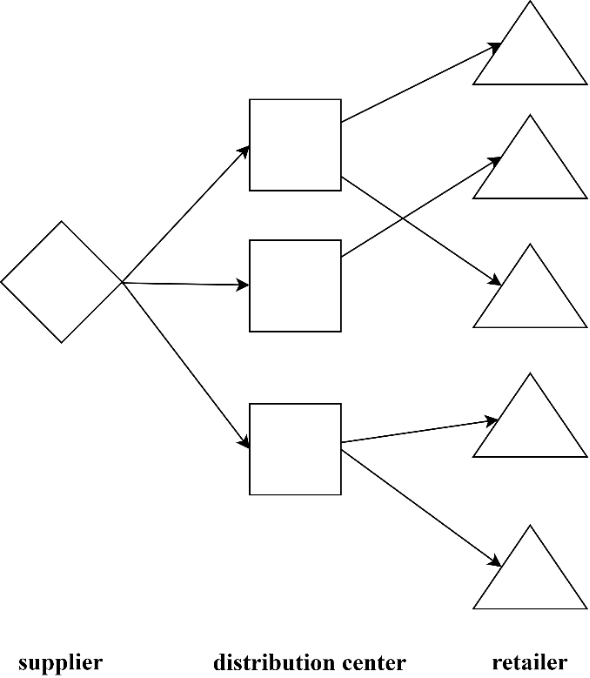
\includegraphics{3-1}
    	\caption{Supply chain network structure diagram}
    	\label{fig:3-1}
    \end{figure}
    
    This study makes several critical assumptions to focus on the core research question. First, retailer demands are independent and follow normal distributions. Each retailer can be served by only one distribution center, and demand cannot be split. Second, we consider only inventory at distribution centers, assuming negligible inventory at retailers. All distribution centers employ an extended Economic Order Quantity (EOQ) model for replenishment, with a uniform service level. This model effectively approximates the (Q, r) inventory policy under a \textit{Type 1 Service Level}. Third, the supplier can respond immediately to replenishment requests, ensuring that lead times are solely determined by transportation and handling processes, not production delays. To focus on the interplay between carbon policy and downstream network design decisions (location, inventory, pricing, carbon trading, and emission reduction investment), we follow common practice in relevant literature and assume that the product's marginal profit is primarily determined by these downstream decisions. Therefore, without loss of generality, we normalize the unit production cost to zero when calculating profits. Fourth, the government permits firms to buy or sell carbon allowances in a cap-and-trade market where the permit price remains constant over the planning horizon. Fifth, firms may invest in a single emission reduction technology, which applies exclusively to distribution center construction, inventory holding, and transportation activities. We do not consider fixed implementation costs for adopting this technology, focusing instead on variable operational costs.
    
    To model this problem, we define the notations in Table \ref{tab:notations}. 
    
    \renewcommand{\arraystretch}{1.25} % 增加行间距的倍数
    \begin{longtable}{p{3.5cm}p{12cm}}
    \caption{Summary of Notations} 
    \label{tab:notations}
    \\
    \toprule
    \textbf{Sets} &  \\
    $J$ & Set of candidate DC locations, indexed by $j$, $|J|=m$ \\
    $I$ & Set of retailers, indexed by $i$, $|I|=n$ \\
    $S_j$ & Set of retailers DC $j$ served, $j\in J $ \\
    \midrule
    \textbf{Parameters} & \\
    $f_j$ & Fixed cost of establishing distribution center $j$, $j\in J$\\
    $F_j$ & Fixed cost for distribution center $j$ to place an order from the supplier, $j\in J$\\
    $L_j$ & Replenishment lead time for distribution center $j$, $j\in J$ (in days)\\
    $h$ & Annual inventory holding cost per unit at the distribution center \\
    $g_j$ & Fixed cost for shipping each order from the supplier to distribution center $j$, $j\in J$ \\
    $a_j$ & The Euclidean distance from the supplier to distribution center $j$, $j\in J$ \\
    $c(a_j)$ & Transportation cost per unit item from the supplier to distribution center $j$, $j\in J$ \\
    $d_{ij}$ & The Euclidean distance from distribution center $j$ to retailer $i$, $j\in J$ , $i\in I$\\
    $c(d_{ij})$ & Transportation cost per unit item from distribution center $j$ to retailer $i$, $j\in J$ , $i\in I$\\
    $\alpha$ & The desired service level for retailer orders \\
    $Z_{\alpha}$ & Standard normal deviation corresponding to the service level, such that: $P(z\leq z_{\alpha})= \alpha$ \\
    $\mu_i$ & Mean annual demand of retailer $i$, $i\in I$ \\
    $\sigma^2_i$ & Variance of daily demand for retailer $i$, $i\in I$ \\
    $D_j$ & Total expected annual demand from the retailers served by distribution center $j$, defined as $D_j=\sum_{i\in S_j}\mu_i$, $ j\in J $\\
    $C$ & Initial carbon emission allowances allocated by the government under cap-and-trade policy \\
    $\hat{f}_j$ & Carbon emissions associated with establishing distribution center $j$, $j\in J$ \\
    $\hat{h}$ & Annual carbon emissions per unit inventory held at the distribution center \\
    $\hat{b}_j$ & Carbon emissions per unit item transported from the supplier to distribution center $j$, $j\in J$ \\
    $\hat{b}_{ij}$ & Carbon emissions per unit item transported from distribution center $j$ to retailer $i$,  $j\in J$ , $i\in I$ \\
    $\hat{p}$ & The price of carbon emission permits in the cap-and-trade market \\
    $v_i$ & Reservation price per unit item for retailer $i$, representing the maximum price the retailer is willing to pay, $i\in I$ \\
    $\theta_j(D_j)$ & Cost coefficient for emission reduction investment for distribution center, $j\in J$ \\
    \midrule
    \textbf{Decision Variables} & \\
    $X_j$ & Equals $1$ if a distribution center is established at candidate location $j$, and $0$ otherwise, $j\in J$\\
    $Y_{ij}$ & Equals $1$ if retailer $i$ is assigned to be served by distribution center $j$ only, and $0$ otherwise, $j\in J$, $i\in I$ \\
    $Q_j$ & Order quantity for distribution center $j$, determined by the EOQ model, $j\in J$\\
    $e^+$ & The quantity of carbon emission permits purchased from the cap-and-trade market within a certain period \\
    $e^-$ & The quantity of carbon emission permits sold in the cap-and-trade market within a certain period \\
    $p_j$ & The wholesale price per unit item set by distribution center $j$ for retailers, $j\in J$. This price affects the range of retailers that can be served by the distribution center \\
    $w_j$ & Carbon emission reduction rate associated with distribution center $j$, with $0\leq w_j\leq 1$, $j\in J$ \\
    \bottomrule
    \end{longtable}
    

    \subsection{Revenue and Cost}
    On the basis of \cite{shen2003joint}  transportation-inventory model and \cite{shen2006profit}'s profit maximization supply chain network design model, this chapter considers the impact of carbon quotas and trading policies and constructs the Cap-and-Trade Supply Chain Network Design (CAT-SCND) model. The model aims to maximize profits, and the objective function is calculated by subtracting the total cost from the total revenue. The total revenue is the total cost of goods paid by the retailer to the distribution center, and the total cost includes the fixed construction cost of the distribution center, the cost of placing orders, the transportation cost of goods, as well as the inventory holding cost and carbon trading cost, all of which are borne by the enterprise. Below, we will take the expenses involved in a distribution center $j$ as an example to provide a detailed introduction to the cost and revenue components of the model. For distribution center $j$, $D_j$ is the sum of the average demand of all retailers it serves, represented as $\sum_{i\in I}\mu_iY_{ij}$.
    
    \begin{itemize}
    
\item\textbf{Total Revenue $\sum_{i\in I}r_i(p_j)\mu_iY_{ij}$:} the revenue gained by distribution center $j$ for servicing retailers $i\in S$, for each $j\in J$. According to the relationship between $p_j$ and $v_i$, the function $r_i(p_j)$ represents the unit revenue obtained by distribution center. This function is a piecewise function as shown in Equation \ref{eq1}. When $p_j$ does not exceed $v_i$, the wholesale price is within the range acceptable to the retailer, forming a service relationship, and the unit revenue of distribution center $j$ from retailer $i$ is $p_j$. When $p_j$ is greater than $v_i$, the wholesale price exceeds the retailer's reservation price, so the retailer will not purchase the product. In other words, the distribution center does not serve that retailer, and the unit revenue of distribution center $j$ from retailer $i$ is $0$. For distribution center $j$, as $p_j$ increases, the unit revenue per item increases, but the number of retailers it can serve decreases, leading to a reduction in the total annual demand $D_j$ covered. Conversely, if $p_j$ decreases, the number of retailers it can serve increases, leading to an increase in the total annual demand $D_j$ covered, but the unit revenue per item decreases. Therefore, the enterprise needs to balance the pricing of goods at each distribution center to determine the set of retailers it can serve, thereby maximizing total profit. 
    \begin{equation}
        \label{eq1}
        r_i(p_j)=\left \{
        \begin{aligned}
            p_j & \quad p_j \leq v_i \\
            0 & \quad p_j > v_i \\  
        \end{aligned}
        \right.
    \end{equation}
    
\noindent\item\textbf{Fixed Facility Location Cost $f_jX_j$:} the facility cost of distribution center $j$ per unit time, for each $j\in J$.

\noindent\item\textbf{Emission Reduction Technology Investment Cost $\frac{1}{2}\delta w^2_j \sqrt{\sum_{i\in I}\mu_iY_{ij}} $:} 
The carbon emission reduction rate at distribution center $j$ is denoted by $w_j \in [0,1]$. Following \cite{dong2016sustainability} and \cite{liu2023study}, the investment cost takes the quadratic form $ \frac{1}{2}\theta_j w^2_j $, where $\theta_j$ is the emission reduction investment cost coefficient. To account for economies of scale and the fact that emission reduction difficulty varies across distribution centers with different demand levels, we define $\theta_j$ as an increasing but concave function of the total demand served: $\theta_j(D_j) = \delta \sqrt{D_j} = \delta \sqrt{\sum_{i\in I}\mu_i Y_{ij}}$, where $\delta$ is a technology-specific constant. This formulation captures that while larger facilities face higher absolute investment costs, they benefit from relatively lower cost increases per unit of demand reduction.
    
\noindent\item\textbf{Transportation Cost $({g_j}/{Q_j}+c(a_j)+c(d_{ij}))\sum_{i\in I}\mu_iY_{ij}$:} an expression that is linear in expected demand rate. The transportation cost of goods can be divided into two parts: transportation from suppliers to distribution centers and transportation from distribution centers to retailers. Among them, a fixed transportation cost $g_j$ is also set for transportation from suppliers to distribution centers. For example, if $c(d_{ij})$ denotes unit transport cost between DC $j$ and retailer $i$, this expression calculates the total annual shipping cost from DC $j$ and the retailers in $S$ that it serves.
    
\noindent\item\textbf{Inventory Replenishment Cost ${F_j\sum_{i\in I}\mu_iY_{ij}}/{Q_j}+{hQ_j}/{2}$:} Inventory replenishment cost involves the turnover inventory and ordering cost of the distribution center. Turnover inventory is determined by the ordering strategy and${Q_j}/{2}$ is the average inventory level between two restocking events in the distribution center $j$. According to the (Q, r) strategy, the cost of placing an order is${F_j\sum_{i\in I}\mu_iY_{ij}}/{Q_j}$.
    
\noindent\item\textbf{Safety Stock Cost $Z_{\alpha}\sqrt{L_j\sum_{i\in I}\sigma_i^2Y_{ij}})$:} within the lead time $L_j$ and meeting the service level $\alpha$, a risk-based expression that is concave and non-decreasing in the total demand variance at DC $j$ and independent demand streams from each retailer that it serves. $\sigma^2_i$ represents variance of daily demand at retailer $i$, for each $i\in I $. This can be used to describe the safety stock cost, and it is concave because of the risk-pooling effect due to demand consolidation at DC $j$. 

\noindent\item\textbf{Carbon trading costs $\hat{p}(e^+-e^-)$:} Among them, $\hat{p}e^+$ represents the cost of purchasing carbon emission quotas for enterprises, and $\hat{p}e^-$ represents the income obtained by enterprises from selling carbon emission quotas. Obviously, at least one of $e^+$ and $e^-$ is 0, indicating that the enterprise purchases or sells carbon emission quotas in the carbon emission trading market, or neither.
    \end{itemize}
    
    
    Based on the above notations, the Cap-and-Trade Supply Chain Network Design (CAT-SCND) model can be formulated as shown in \textbf{Model-}$\Pi_\kappa$.
    
    \begin{align}
    & \textbf{Model-} \Pi_\kappa & & \notag\\
    & \max        & & \notag\\
    & & &\sum_{j\in J} \Big[ \sum_{i\in I}r_i(p_j)\mu_iY_{ij}-f_jX_j-\frac{1}{2}\delta w^2_j \sqrt{\sum_{i\in I}\mu_iY_{ij}}\notag  \\
    & & &-(\frac{F_j+g_j}{Q_j}+c(a_j)+c(d_{ij}))\sum_{i\in I}\mu_iY_{ij} \notag  \\
    & & &-\frac{hQ_j}{2}-hz_{\alpha} \sqrt{L_j\sum_{i\in I}\sigma^2_iY_{ij}} \Big]-\hat{p}(e^+-e^-) \label{obj:3-1}\\
    & \mbox{subject to} && \notag  \\
    & & & \sum_{j\in J}\Bigg[(\hat{f}_jX_j+\hat{h}(\frac{Q_j}{2}+z_{\alpha}\sqrt{L_j\sum_{i\in I}\sigma^2_iY_{ij}}) \notag  \\
    & & &+\sum_{i\in I}(\hat{b}_j+\hat{b_{ij}})\mu_iY_{ij})(1-w_j)\Big] \notag \\
    & & &+(e^--e^+)=C  \label{cons:3-1}\\
    & & &\quad\quad \sum_{j\in J}Y_{ij} \leq 1, \forall{i\in I} \label{cons:3-2}\\
    & & &\quad\quad Y_{ij} \leq X_j ,  \forall{i\in I}, \forall{j\in J} \label{cons:3-3}\\
    & & &\quad\quad Q_j \geq 0, \forall{j\in J} \label{cons:3-4}\\
    & & &\quad\quad p_j \geq 0, \forall{j\in J} \label{cons:3-5}\\
    & & &\quad\quad 0 \leq w_j \leq 1, \forall{j\in J} \label{cons:3-6}\\
    & & &\quad\quad Y_{ij} \in \{0,1\} ,  \forall{i\in I}, \forall{j\in J} \label{cons:3-7}\\
    & & &\quad\quad X_{j} \in \{0,1\} ,  \forall{j\in J} \label{cons:3-8}\\
    & & &\quad\quad e^+ \geq 0 \label{cons:3-9}\\
    & & &\quad\quad e^- \geq 0 \label{cons:3-10}
    \end{align}
    
    The objective function (\ref{obj:3-1}) of the model calculates the total revenue minus the total cost. The total revenue is the total amount paid by retailers to the distribution centers for goods. The total cost includes the fixed construction costs of the distribution centers, ordering costs, transportation costs of goods, inventory holding costs, carbon trading costs, and emission reduction technology investment costs, all of which are borne by the enterprise.

    \textbf{Note on inventory cost formulation:} In the objective function (\ref{obj:3-1}), the inventory holding cost is expressed as $(h+\hat{p}\hat{h}(1-w_j))\left(\frac{Q_j}{2}+z_{\alpha} \sqrt{L_j\sum_{i\in I}\sigma^2_iY_{ij}}\right)$. This unified term combines both the cycle stock cost (from average inventory $Q_j/2$) and the safety stock cost (from $z_{\alpha} \sqrt{L_j\sum_{i\in I}\sigma^2_iY_{ij}}$), each adjusted for both financial holding cost ($h$) and carbon emissions cost ($\hat{p}\hat{h}(1-w_j)$). While we separately described these components in Section 3.1 for conceptual clarity, their combined formulation here reflects that both types of inventory incur identical per-unit holding and carbon costs in practice. This consolidation simplifies the mathematical expression while maintaining economic and environmental cost accuracy.
    
     Constraint (\ref{cons:3-1}) is the limit on the total carbon emissions of the enterprise under cap-and-trade policy. In the supply chain network studied in this paper, carbon emissions primarily come from three aspects: the construction of distribution centers, the transportation of goods, and inventory holding. These emissions are borne by the enterprise that owns the suppliers and distribution centers. The enterprise bases its carbon emissions on the emissions after implementing emission reduction technologies. According to cap-and-trade policy, any shortage or surplus of carbon emission allowances can be offset or profited through carbon trading. If the total carbon emissions exceed the initial carbon emission allowance, the enterprise needs to purchaseunits of carbon emission allowances in the carbon trading market. Conversely, if the total carbon emissions are less than, up tounits of carbon emission allowances can be sold to generate income. Clearly, to maximize profit, the enterprise will sell all unused carbon emission allowances.
     Constraint (\ref{cons:3-2}) stipulates that a retailer can be served by at most one distribution center. Constraint (\ref{cons:3-3}) indicates that retailers can only be assigned to an established distribution center. Constraints (\ref{cons:3-4}) and (\ref{cons:3-5}) ensure that the order quantity and wholesale price of goods meet the non-negative requirements. Constraints (\ref{cons:3-6}) specifies the range of the emission reduction rate. Constraints (\ref{cons:3-7}) and (\ref{cons:3-8}) are standard integer programming constraints. Constraints (\ref{cons:3-9}) and (\ref{cons:3-10}) impose non-negative restrictions on the quantity of carbon emission allowances the enterprise can buy and sell.
    
    \subsection{Model Reformulation}
    To simplify the model, use the notation $e^+-e^-$ based on constraint $(3)$, and substitute it in the same part of the objective function. The objective function can then be rewritten as Equation \ref{eq2}. In the transformed objective function, $e^+$ and $e^-$ do not appear, indicating that carbon trading decisions do not affect other decisions in supply chain network design. The final outcome of carbon trading decisions is calculated based on the enterprise's carbon emissions $E$ and the initial carbon emission cap $C$ when maximizing profit, i.e., $e^+=max\{ E-C, 0\},e^-=max\{ C-E, 0\}$.
    
   \begin{align}
    \label{eq2}
    & \max  & &  
    \sum_{j\in J} \Big[ \sum_{i\in I}r_i(p_j)\mu_iY_{ij}-(f_j+\hat{f}_j\hat{p}(1-w_j))X_j \notag \\
     & & &-\frac{1}{2}\delta w^2_j \sqrt{\sum_{i\in I}\mu_iY_{ij}}-\sum_{i\in I}(c(d_{ij})+\hat{p}\hat{b}_{ij}(1-w_j))\mu_iY_{ij}  \notag \\
     & & & -(h+\hat{p}\hat{h}(1-w_j))(\frac{Q_j}{2}+z_{\alpha} \sqrt{L_j\sum_{i\in I}\sigma^2_iY_{ij}}) \notag\\
     & & &-(\frac{F_j+g_j}{Q_j}+c(a_j)+\hat{p}\hat{b}_j(1-w_j))\sum_{i\in I}\mu_iY_{ij} \Big]+\hat{p}C 
\end{align}
    
    In situations where demand uncertainty exists for retailers, the (Q, r) model can be considered to supplement inventory. This model implies ordering $Q$ units of inventory when the inventory level drops to units. \cite{zhang1992properties} and \cite{axsater1996using} have shown that under the first-class service level, the EOQ model can effectively approximate the $(Q, r)$ model with an error not exceeding 0.118. Therefore, in this study, the distribution centers use the EOQ model for replenishment. Taking into account the introduction of carbon emissions in the model, an extended EOQ model is employed to determine the optimal order quantity $Q^*_j$, for distribution center $j$, as shown in Equation \ref{eq3}.
    
    \begin{align}
        \label{eq3}
        Q_j^*=\sqrt{\frac{2(F_j+g_j)\sum_{i\in I}\mu_iY_{ij}}{h+\hat{p}\hat{h}(1-w_j)}}
    \end{align}
    
    The transformed \textbf{Model-}$\Pi_\chi$ is as follows:
    
    \begin{align}
    \label{model2}
    & \textbf{Model-} \Pi_\chi & & \notag\\
    & \max        & & \notag\\
    & & &\sum_{j\in J} \Big[ \sum_{i\in I}r_i(p_j)\mu_iY_{ij}-(f_j+\hat{f}_j\hat{p}(1-w_j))X_j \notag  \\
    & & &-\sum_{i\in I}(c(d_{ij})+\hat{p}\hat{b}_{ij}(1-w_j))\mu_iY_{ij} 
    -\frac{1}{2}\delta w^2_j \sqrt{\sum_{i\in I}\mu_iY_{ij}}\notag  \\
    & & &-(h+\hat{p}\hat{h}(1-w_j))z_{\alpha} \sqrt{L_j\sum_{i\in I}\sigma^2_iY_{ij}}
    \notag  \\
    & & &-\sqrt{2({F_j+g_j})(h+\hat{p}\hat{h}(1-w_j))\sum_{i\in I}\mu_iY_{ij}} \notag  \\
    & & &-(c(a_{j})+\hat{p}\hat{b}_j(1-w_j))\sum_{i\in I}\mu_iY_{ij}  \Big]+\hat{p}C \\
    & \mbox{subject to} && \notag  \\
    & & &\quad\quad \sum_{j\in J}Y_{ij} \leq 1, \forall{i\in I} \\
    & & &\quad\quad Y_{ij} \leq X_j ,  \forall{i\in I}, \forall{j\in J} \\
    & & &\quad\quad p_j \geq 0, \forall{j\in J} \\
    & & &\quad\quad 0 \leq w_j \leq 1, \forall{j\in J} \\
    & & &\quad\quad Y_{ij} \in \{0,1\},  \forall{i\in I}, \forall{j\in J} \\
    & & &\quad\quad X_{j} \in \{0,1\} ,  \forall{j\in J} 
    \end{align}
    
    Due to the introduction of the decision variable $w_j$ in model $\Pi_\chi$, involving the multiplication of binary $(0-1)$ and continuous variables, along with the consideration of the impact of emission reduction technology investment costs, the structure and nature of the model become more complex. Considering the difficulty of accurately solving such problems, this paper proposes a hybrid genetic algorithm with branch-and-price for solution.
    
    
    \section{Solution Approach}
    The hybrid genetic algorithm proposed in this paper combines genetic algorithms with other optimization techniques. The genetic algorithm component employs an elitist strategy, which preserves the best individuals in each generation, thereby preventing the loss of the best solution during selection, crossover, and mutation processes. \cite{rudolph1994convergence} demonstrated through Markov chain theory that a genetic algorithm using only selection, crossover, and mutation operations may not converge to the global optimum, whereas an elitist strategy ensures global convergence. For other optimization techniques, such as the branch-and-price algorithm, the choice depends on the specific problem characteristics. The branch-and-price algorithm theoretically guarantees the optimal solution, but its practical application may be limited by problem complexity.  By integrating the genetic algorithm's global search capability with the local search capability of other optimization techniques, the hybrid approach effectively addresses complex optimization problems in the model. The introduction of the elitist strategy enhances algorithm convergence and stability, mitigating the risk of getting trapped in local optima and accelerating the genetic algorithm's convergence towards an approximate optimum solution.
    
    \subsection{Hybrid Genetic Algorithm}
    
    This subsection introduces the hybrid genetic algorithm. In \textbf{Model-}$\Pi_\chi$, only the decision variables $w_j(j\in J)$ are encoded in the genetic encoding part. If the values of variables $w_j(j\in J)$  are known, there will be no multiplication of continuous and 0-1 variables in the model. At this point, the model can be transformed into a set-covering model, which can be solved using a branch-and-price algorithm. This encoding strategy, focusing only on $w_j(j\in J)$ rather than all decision variables, allows the problem to quickly obtain a better solution in the early iterations of genetic iteration. As the genetic algorithm iterates multiple rounds, the maximum fitness gradually converges, eventually yielding an approximate optimal solution.
    Before starting the genetic algorithm, it is necessary to set the relevant parameters, including population size, crossover probability, mutation probability, and maximum number of iterations. Proper parameter settings can effectively improve the performance and convergence speed of the genetic algorithm, thereby better solving the optimization problem.
    The genetic algorithm with an elite preservation strategy is similar to traditional genetic algorithms, with some improvements in certain steps. The specific process is as follows:
    \begin{enumerate}[label=(\arabic*), parsep=0pt, itemsep=10pt, leftmargin=*, itemindent=2em]
        \item \textbf{Initialization of the population:} 
    Initialize a population where each individual represents a solution for $w_j(j\in J)$. The decision variables $w_j(j\in J)$ are encoded in binary format. Considering that $w_j$ is a continuous variable in the range $[0,1]$, to ensure precision, the interval $[0,1]$ is divided. Assuming retention to $n$ decimal places, the length $l_j$ of the binary string representing $w_j$ can be chosen as the smallest positive integer m satisfying $2^m-1 \geq 10^n$. Each $w_j$ is represented by a binary string of length $l_j$, and the length of a binary string for an individual is $l_j \times  |J|$, as shown in Figure \ref{fig:4-1}.
    \begin{figure}
    	\centering
    	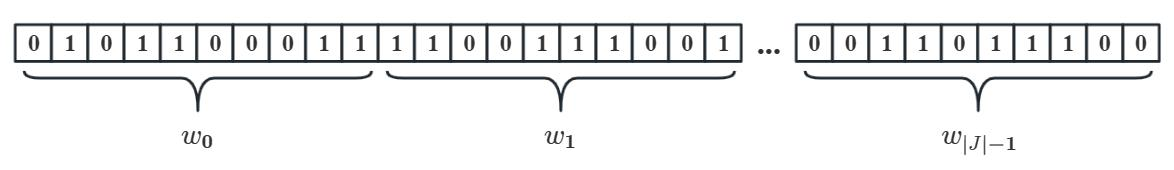
\includegraphics{4-1}
    	\caption{Individual schematic}
    	\label{fig:4-1}
    \end{figure}
        \item \textbf{Fitness evaluation:}
    Before calculating fitness, individuals need to be decoded. Decode the binary string corresponding to , converting it into decimal form using the formula $w_j=decimal(substring_j)/(2^{l_j}-1)$, where $substring_j$ is the binary substring corresponding to $w_j$, and $decimal(\cdot)$ is the decimal conversion function. Considering that the objective of this chapter's model is profit maximization and, according to the model's nature, function values cannot be negative, the objective function can be directly set as the fitness function, where the objective function value is the fitness value. To obtain the objective function value, the model needs to be transformed into a set covering model, and then solved using the branch-and-price algorithm.
        \item \textbf{Elite preservation:}
    The individual with the highest fitness value is directly copied to the next generation to ensure its presence in the new generation.
        \item \textbf{Selection:}
    Parent selection is performed using the roulette wheel selection method to choose individuals with higher fitness values. In the roulette wheel selection method, the probability of each individual being selected is proportional to its fitness value relative to the total fitness value of all individuals in the population. Let $f_k$ be the fitness value of the $k-th$ individual in the population of size $N$, and let $p_k$ represent the probability of the $k-th$ individual being selected, as expressed in Equation (\ref{eq:4-1}). The higher the fitness value, the greater the probability of being selected. The specific steps of the roulette wheel selection method are as follows: First, for each individual in the population, calculate the ratio of its fitness value to the sum of fitness values of all individuals in the population according to Equation \ref{eq:4-1}. Then, divide the roulette wheel into corresponding sectors based on this ratio. Rotate a random pointer on the roulette wheel, and the pointer stops in the sector corresponding to the selected individual. Repeat this process until a sufficient number of parent individuals are selected.
    \begin{align}
        \label{eq:4-1}
        p_k=\frac{f_k}{\sum^N_{k=1}f_k}
    \end{align}
        \item \textbf{Crossover:}
    Based on the crossover probability, it is determined whether to perform the crossover operation. In this chapter, a two-point crossover method is employed, where two crossover points are randomly generated. Only the genes between the crossover points of the parent individuals are exchanged, as illustrated in Figure \ref{fig:4-2}.

\begin{figure}[htbp]
    \centering
    \begin{subfigure}{0.45\textwidth}
        \centering
        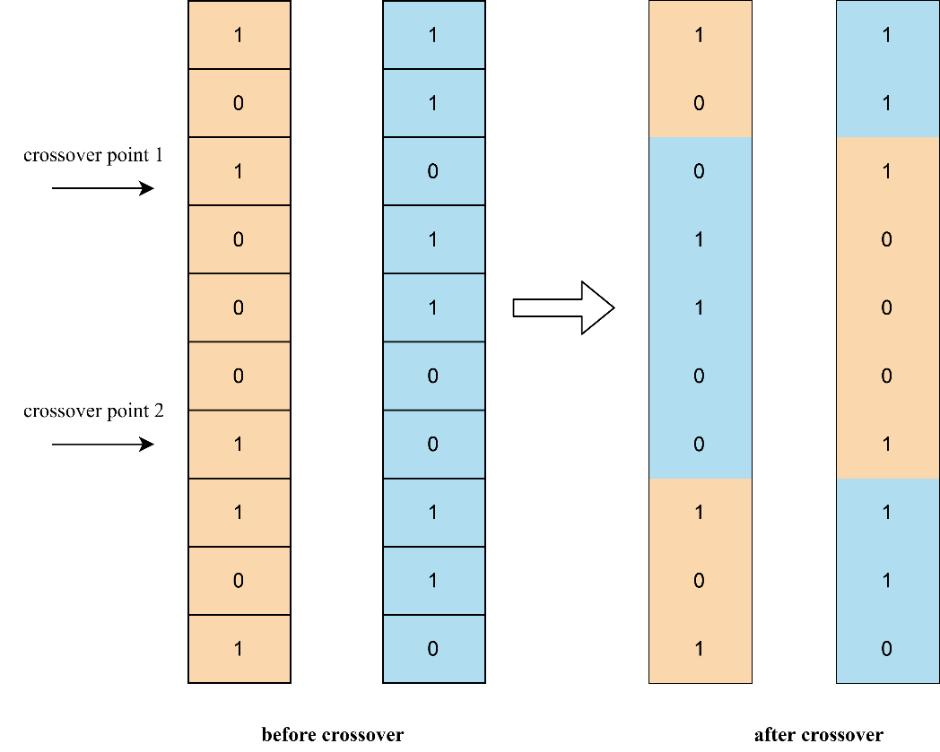
\includegraphics[width=\linewidth]{4-2}
        \caption{Schematic of two-point crossover}
        \label{fig:4-2}  
    \end{subfigure}
    \hfill
    \begin{subfigure}{0.45\textwidth}
        \centering
        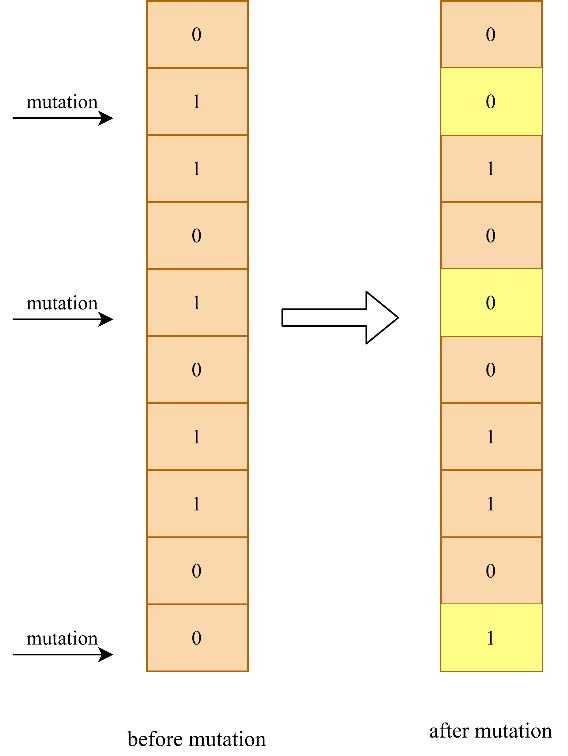
\includegraphics[width=0.8\linewidth, height=0.8\linewidth]{4-3}
        \caption{Schematic of individual variation}
        \label{fig:4-3}  
    \end{subfigure}
    \label{fig:4-2&3}
\end{figure}
    
        \item \textbf{Mutation:}
    For individuals encoded in binary format, each binary bit of the individual is traversed. According to the mutation probability, the binary bits corresponding to the genes of the parent individual are directly reversed, meaning 0 becomes 1 and 1 becomes 0, as depicted in Figure \ref{fig:4-3}.
    
        \item \textbf{Update Population:}
    Combine the individuals with the highest fitness values from the previous round with the offspring to form the new population.
        \item \textbf{Repeat Iteration:}
    Repeat steps (2) to (7) until the stopping criteria are met, such as reaching the maximum number of iterations or the optimal fitness value remains unchanged after multiple iterations.    
    \end{enumerate}
    
    
    \subsection{Branch-and-Price Algorithm}
    The above genetic algorithm with elitism outlines the overall approach for solving the model. In the fitness evaluation module, the objective function value of the model needs to be obtained. After obtaining the carbon emission reduction rate $w_j(j\in J)$ through genetic encoding, the model can be equivalently transformed into a set-covering model. This transformation introduces a massive number of decision variables (up to $2^{|I|\times |J|}$), rendering conventional integer programming solvers ineffective. To tackle this computational challenge, we employ the \textbf{Branch-and-Price} algorithm.
    
    \subsubsection{The Set-Covering Formulation and Master Problems}
    
    First, we define the necessary components for the set-covering formulation:
    Define $\bar{R}_{j,S}$, which represents the net profit of distribution center $j$ serving the set $S$ of retailers considering carbon emissions and investment costs in emission reduction technologies, as shown in Equation \ref{eq:4-2}. Then introduce the binary variable $\bar{Z}_{j,S}$. When $\bar{Z}_{j,S}=1$, it indicates that distribution center $j$ serves the set of retailers $S$; otherwise, $\bar{Z}_{j,S}=0$. Here, $j\in J$, $S\subseteq I$.
    
    \begin{equation}
    \begin{aligned}
        \label{eq:4-2}
        \bar{R}_{j,S} &= 
        \sum_{i\in S}r_i(p_j)\mu_i-(f_j+\hat{f}_j\hat{p}(1-w_j))  -\sum_{i\in S}\big(c(d_{ij})+\hat{p}\hat{b}_{ij}(1-w_j)\big)\mu_i \\
        &\quad -\frac{1}{2}\delta w^2_j \sqrt{\sum_{i\in S}\mu_i}  -(h+\hat{p}\hat{h}(1-w_j))z_{\alpha} \sqrt{L_j\sum_{i\in S}\sigma^2_i} \\
        &\quad -\sqrt{2({F_j+g_j})(h+\hat{p}\hat{h}(1-w_j))\sum_{i\in S}\mu_i Y}  -\big(c(a_{j})+\hat{p}\hat{b}_j(1-w_j)\big)\sum_{i\in S}\mu_i 
    \end{aligned}
    \end{equation}
    
    
    
    The integer master problem (\textbf{Model-}$\Pi_M$) and its linear relaxation (\textbf{Model-}$\Pi_{LM}$) are constructed as follows:
    \begin{align}
    \label{model3}
    & \textbf{Model-} \Pi_M & \max    & \sum_{j\in J} \sum_{S\in I}\bar{R}_{j,S}\bar{Z}_{j,S}+\hat{p}C  &\\
    & \mbox{subject to} && \sum_{j\in J}\sum_{S\subseteq I:i\in S} \bar{Z}_{j,S} \leq 1, \forall{i\in I} &\\
    &&& \sum_{S\subseteq I} \bar{Z}_{j,S} \leq 1,   \forall{j\in J} & \label{cons:4-3}\\
    &&& \bar{Z}_{j,S} \in \{0,1\},  \forall{j\in J}, \forall{S\subseteq I} &
    \end{align}
    
    
    \begin{align}
    \label{model4}
    & \textbf{Model-} \Pi_{LM} & \max    & \sum_{j\in J} \sum_{S\in I}\bar{R}_{j,S}\bar{Z}_{j,S}+\hat{p}C  &\\
    & \mbox{subject to} && \sum_{j\in J}\sum_{S\subseteq I:i\in S} \bar{Z}_{j,S} \leq 1, \forall{i\in I} &\\
    &&& \sum_{S\subseteq I} \bar{Z}_{j,S} \leq 1,   \forall{j\in J} &\\
    &&& 0 \leq \bar{Z}_{j,S} \leq 1 ,  \forall{j\in J}, \forall{S\subseteq I} &
    \end{align}
    
    Constraint (\ref{cons:4-3}) ensures the consistency of the wholesale price $p_j$ for the same product from the same distribution center $j$. After converting to a set-covering model, both the objective function and constraints do not contain non-linear terms. Considering that \textbf{Model-}$\Pi_M$ belongs to the realm of integer programming with an exponential number of variables, we now present the Branch-and-Price algorithm specifically designed to solve it.
    
    \subsubsection{The Branch-and-Price Algorithm Framework}
    
    Branch-and-Price is an advanced optimization framework that synergistically combines two powerful methodologies:
    
    \textbf{Branch and Bound (B\&B)}: A strategic tree search algorithm that systematically partitions the solution space to enforce integrality constraints and find the optimal integer solution.
    
    \textbf{Column Generation (CG)}: An efficient algorithm for solving the linear programming (LP) relaxations of problems with a huge number of variables by dynamically generating only the most promising ones.
    
    The overall Branch-and-Price framework works as follows (See Algorithm \ref{alg:bp}). At each node of the tree, the LP relaxation is solved not by a standard solver, but by the CG algorithm. This integrated approach is essential for handling the exponentially sized model we face.
    
    \begin{breakablealgorithm}
    \small
    \renewcommand{\baselinestretch}{1.2}\selectfont 
    \caption{Branch-and-Price Algorithm for \textbf{Model-}$\Pi_M$}
    \label{alg:bp}
    \begin{algorithmic}[1]
    \State \textbf{Initialization:}
    \State \qquad Create the \textbf{Root Node} of the B\&B tree, the linear relaxation problem \textbf{Model-}$\Pi_{LM}$.
    \State \qquad Initialize the \textit{activeNodes} list with the \textbf{Root Node}.
    \State \qquad Set the \textbf{Best Integer Solution} (incumbent) to $\emptyset$.
    \State \qquad Set the global \textbf{Lower Bound (LB)} to $-\infty$.
    \State \textbf{While} \textit{activeNodes} is not empty \textbf{do}
    \State \qquad \textbf{Step 1: Node Selection}: Select and remove a node $N$ from \textit{activeNodes}.
    \State \qquad \textbf{Step 2: Bound}: Solve the LP relaxation of node $N$ using the \textbf{Column Generation} procedure.
    \State \qquad \qquad Let $z_N$ be the optimal objective value and $\mathbf{\bar{Z}}$ the solution.
    \State \qquad \textbf{Step 3: Pruning}:
    \State \qquad \qquad \textbf{If} (infeasible) \textbf{then} \textbf{prune} (fathom) the node. \textbf{// Prune by Infeasibility}
    \State \qquad \qquad \textbf{Else If} ($z_N^* \leq$ LB) \textbf{then} \textbf{prune} the node. \textbf{// Prune by Bound}
    \State \qquad \qquad \textbf{Else If} ($\mathbf{\bar{Z}}$ is integer) \textbf{then}
    \State \qquad \qquad \qquad Update incumbent and LB = $z_N$ if $z_N^* >$ LB.
    \State \qquad \qquad \qquad \textbf{prune} the node. \textbf{// Prune by Optimality}
    \State \qquad \qquad \textbf{Else}
    \State \qquad \qquad \qquad \textbf{Step 4: Branch}:
    \State \qquad \qquad \qquad Choose a fractional variable $\bar{Z}_{j', S'}$ from $\mathbf{\bar{Z}}^*$.
    \State \qquad \qquad \qquad Create two new child nodes:
    \State \qquad \qquad \qquad - Node $N_1$: add constraint $\bar{Z}_{j', S'} = 0$
    \State \qquad \qquad \qquad - Node $N_2$: add constraint $\bar{Z}_{j', S'} = 1$
    \State \qquad \qquad \qquad Add $N_1$ and $N_2$ to \textit{activeNodes}.
    \State \qquad \qquad \textbf{End If}
    \State \textbf{End While}
    \State \textbf{Return:} The incumbent solution.
    \end{algorithmic}
    \end{breakablealgorithm}  
    
    \subsubsection{Column Generation for Solving Linear Relaxations}
    Column generation is an optimization algorithm designed to solve large-scale linear programming problems by dynamically generating variables (columns) rather than enumerating all possibilities explicitly. This method starts with a small subset of columns in a Restricted Master Problem (RMP), iteratively solves it, and uses its dual solution to identify new columns with the potential to improve the objective function. We adopt this algorithm to solve the linear relaxation \textbf{Model-}$\Pi_{LM}$ of our problem.
    
    The RMP, denoted as \textbf{Model-}$\Pi_{RM}$, is defined with a restricted set $W$ of retailer subsets ($W \subseteq 2^I$):
    \begin{align}
    \label{model5}
    & \textbf{Model-} \Pi_{RM} & \max    & \sum_{j\in J} \sum_{S\in W}\bar{R}_{j,S}\bar{Z}_{j,S}+\hat{p}C  &\\
    & \mbox{subject to} && \sum_{j\in J}\sum_{S\subseteq W:i\in S} \bar{Z}_{j,S} \leq 1, \forall{i\in I} &\\
    &&& \sum_{S\subseteq W} \bar{Z}_{j,S} \leq 1,   \forall{j\in J} &\\
    &&& 0 \leq \bar{Z}_{j,S} \leq 1 ,  \forall{j\in J}, \forall{S\subseteq W} &
    \end{align}
    
    The column generation procedure iterates as follows:
    \begin{enumerate}
    \item\textbf{Solve the RMP}: The current \textbf{Model-}$\Pi_{RM}$ is solved, yielding the primal solution $\bar{Z}^*_{j,S}$ and, crucially, the dual solution $\bar{\lambda}_i$ ($\forall i \in I$) and $\bar{\lambda}_{|I|+j}$ ($\forall j \in J$).
    
    \item\textbf{Solve the Pricing Subproblem}: The dual solution is used to formulate a pricing subproblem. The goal is to find a new column $(j, S)$, a facility-retailer-set pair, with a positive reduced cost, indicating that adding this column to the RMP could improve the objective value. The reduced cost for a column $(j, S)$ is given by:
    $\bar{R}_{j,S} - \sum_{i\in S}\bar{\lambda}_i - \bar{\lambda}_{|I|+j}$.
    Therefore, for each facility $j \in J$, we define the pricing subproblem:
    \begin{align}
    \label{model6}
    & \textbf{Model-} SM_{j} & \max_{S\subseteq I}    & \bar{R}_{j,S}-\sum_{i\in S}\bar{\lambda}_i-\bar{\lambda}_{|I|+j}  &
    \end{align}
    
    
    \item\textbf{Check Optimality \& Update}: If no column with a positive reduced cost is found across all $j \in J$ ($\max_j(SM_j) \leq 0$), the current solution of the RMP is also optimal for the full linear relaxation \textbf{Model-}$\Pi_{LM}$, and the algorithm terminates. Otherwise, the column with the maximum positive reduced cost is added to the restricted set $W$, and the process repeats.
    \end{enumerate}
    
    A significant complication in our problem is that the wholesale price $p_j$ is a decision variable within $\bar{R}_{j,S}$, making the pricing subproblem a complex, joint optimization over $S$ and $p_j$. To solve \textbf{Model-}$SM{j}$, we must find the triple $(j, S, p_j)$ that maximizes the reduced cost. Fortunately, the pricing decision exhibits a favourable structure. Based on the research by \cite{shen2006profit} and \cite{li2014stochastic}, the optimal price $p_j^*$ for any facility $j$ is not arbitrary but is guaranteed to be one of the reservation prices of the retailers.
    
    
    \begin{theorem} \label{thm:price_structure}
    Let $S^*$ and $p_j^*$ be the optimal retailer set and wholesale price for facility $j$ in \textbf{Model-}$SM_{j}$, respectively. If $S^*$ is non-empty, then $p_j^* \in \{v_i \mid i \in S_j \}$, where $v_i$ is the reservation price of retailer $i$, $S_j$ is the retailer set served by DC $j$.
    \end{theorem}
    
    
    This theorem simplifies the pricing subproblem immensely. It allows us to solve \textbf{Model-}$SM_{j}$ by enumerating a finite set of candidate prices $p_j \in \{v_i | i \in S_j\}$. For each candidate price, $p_j$ is fixed, and we solve a simpler subproblem to find the best retailer set $S^*(p_j)$. The overall best solution $(S^*, p_j^*)$ is the one with the highest reduced cost across all candidate prices. The overall column generation algorithm incorporating this pricing strategy is summarized in Algorithm \ref{alg-cg}. And the detailed algorithm for solving this subproblem is the focus of the next section. 
    \begin{breakablealgorithm} 
    \small
    \renewcommand{\baselinestretch}{1.2}\selectfont 
    \caption{Column Generation Algorithm for \textbf{Model-}$\Pi_{RM}$}
    \label{alg-cg}
    \begin{algorithmic}[1]
    \State \textbf{Initialize:} Construct the RMP (\textbf{Model-}$\Pi_{RM}$) with an initial set $W$ of columns.
    \Repeat
    \State Solve the RMP to obtain the primal solution $\bar{Z}^*$ and dual values $\bar{\lambda}^*$.
    \State $rc^*_{max} \gets -\infty$ \Comment{Initialize the maximum reduced cost}
    \State $j^* \gets \emptyset$, $S^* \gets \emptyset$, $p_j^* \gets \emptyset$ \Comment{Initialize the best column}
    \For{each facility $j \in J$} \Comment{Outer loop: iterate over facilities}
        \For{each candidate price $p_j$ in the set $\{v_i \mid i \in S_j\}$} \Comment{Iterate over candidate prices}
            \State Solve \textbf{Model-}$SM_j(p_j)$: $\max_{S \subseteq I} \{ \bar{R}_{j,S}(p_j) - \sum_{i\in S}\bar{\lambda}_i - \bar{\lambda}_{|I|+j} \}$
            \State Let $(S_j, rc_j)$ be the solution \Comment{Find best $S$ for this $p_j$}
            \If{$rc_j > rc^*_{max}$}
                \State $rc^*_{max} \gets rc_j$
                \State $j^* \gets j$
                \State $S^* \gets S_j$
                \State $p_j^* \gets p_j$ \Comment{Record the best price found so far}
            \EndIf
        \EndFor
    \EndFor
    \If{$rc^*_{max} > 0$}
        \State $W \gets W \cup \{(j^*, S^*)\}$ \Comment{Add the best column $(j, S)$ to RMP}
    \EndIf
    \Until{$rc^*_{max} \leq 0$} \Comment{Terminate if no profitable column exists}
    \State \textbf{Return:} The optimal solution $\bar{Z}^*$ for \textbf{Model-}$\Pi_{LM}$.
    \end{algorithmic}
\end{breakablealgorithm}
    
    
    
    \subsection{Pricing subproblem}
    
    The efficiency of the column generation algorithm hinges on the effective solution of the pricing subproblem \textbf{Model-}$SM_{j}$ for each facility $j$. As established, Theorem \ref{thm:price_structure} allows us to determine the optimal price $p_j^*$ by evaluating a finite set of candidate values. This section details the method for solving \textbf{Model-}$SM_{j}$ for a given $j$ and a fixed candidate price $p_j$.
    
    
    For a given facility $j$ and fixed price $p_j$, we reformulate \textbf{Model-}$SM_j$ based on Equation \ref{eq:4-2}. The pricing subproblem can be expressed as:
    
    
    \begin{align}
    \label{model7}
    & \textbf{Model-} SM_{j}(p_j) & \min_{S\subseteq I}\quad    &\sum_{i\in S}\bar{A}_i(p_j)+\bar{G}_j(\sum_{i\in S}\mu_i)+\bar{K}_j(\sum_{i\in S}\sigma^2_i) +(f_j+\hat{f}_j\hat{p}(1-w_j))+\bar{\lambda}_{|I|+j}&\\
    &&where, \quad &\bar{A}_i(p_j)=\big( c(d_{ij})+\hat{p}\hat{b}_{ij}(1-w_j)+c(a_j)+\hat{p}\hat{b}_j(1-w_j)-r_i(p_j) \big)\mu_i+\bar{\lambda}_i &\\
    && & \bar{G}_j(\sum_{i\in S}\mu_i)=(\sqrt{2(F_j+g_j)(h+\hat{p}\hat{h}(1-w_j)}+\frac{1}{2}\delta w_j^2)\sqrt{\sum_{i\in S}\mu_i}\\
    && &\bar{K}_j(\sum_{i\in S}\sigma^2_i)=(h+\hat{p}\hat{h}(1-w_j))Z_\alpha\sqrt{L_j\sum_{i \in S}\sigma^2_i}
    \end{align}
    
    
    Since the constant term $(f_j+\hat{f}_jp(1-w_j))+\bar{\lambda}_{|I|+j}$  does not affect the optimization over $j$, we can ignore it and focus on the simplified problem:
    
    \begin{align}
    \label{model8}
    & \textbf{Model-} SM^{\prime}_{j}(p_j) & \min_{S\subseteq I}\quad    &\sum_{i\in S}\bar{A}_i(p_j)+\bar{G}_j(\sum_{i\in S}\mu_i)+\bar{K}_j(\sum_{i\in S}\sigma^2_i)&
    \end{align}
    
    The solution space of \textbf{Model-}$SM^{\prime}_j(p_j)$ contains $2^{|I|}$ possible retailer sets, making exhaustive search computationally prohibitive for large instances. To obtain the optimal solution in polynomial time, we employ the parametric linear programming technique following the work of \cite{chakravarty1985consecutive}, \cite{shu2005stochastic}, and \cite{shu2011market}. Due to the concavity of $\bar{G}_j$ and $\bar{K}_j$, the optimal solution must lie on the convex hull of the set of all feasible points in this three-dimensional space. This structural property allows us to efficiently search for the optimal solution by considering only a polynomial number of candidate sets. Algorithm \ref{alg-pb} implements the parametric programming approach for solving \textbf{Model-}$SM^{\prime}_j(p_j)$. 
    
    \begin{breakablealgorithm}  
        \small
        \renewcommand{\baselinestretch}{1.2}\selectfont 
        \caption{Parametric Programming Algorithm for \textbf{Model-}$SM^{\prime}_j(p_j)$} 
        \label{alg-pb}
        \begin{algorithmic}[1]
            \State \textbf{Initialize:} $R_p,R_q,I_1,I_2,I_3,S^* \gets \varnothing, num\gets 0, I^-[\ ]$ 
            \State \textbf{Step 1: Preprocess retailers and compute features}
            \For{$i=1$ \textbf{to} $|I|$}
                \State $e_i^{\prime}\gets \bar{A}_i(p_j)$
                \If {$e_i^{\prime}<0$} 
                    \State $I^-[num]\gets i$, $num \gets num+1$
                    \State $e_{num}\gets e_i^{\prime}$ 
                    \State $g_{num}\gets \bar{G}_j(\sum_{i\in I^-}\mu_i)$ 
                    \State $k_{num}\gets \bar{K}_j(\sum_{i\in I^-}\sigma^2_i)$ 
                    \State $x_{num} \gets -{k_{num}}/{e_{num}}$, $y_{num} \gets -{g_{num}}/{e_{num}}$ 
                \EndIf
            \EndFor
            
            \State \textbf{Step 2: Explore candidate partitions}
            \For {$p=1$ \textbf{to} $num-1$}
                \For {$q=p+1$ \textbf{to} $num$}
                    \State \textbf{def:} $\vec{pq} \gets (x_q-x_p,y_q-y_p)$ \Comment{Direction vector between points}
                    \State \textbf{def:} $\cos(\vec{p},\vec{q}) \gets \dfrac{x_px_q+y_py_q}{\sqrt{x_p^2+y_p^2}\sqrt{x_q^2+y_q^2}}$ \Comment{Cosine similarity}
                    
                    \If {$x_p = x_q$ \textbf{and} $y_p = y_q$} \Comment{Skip identical points}
                        \State \textbf{continue}
                    \EndIf
                    
                    \State \textbf{Define partitioning function} $F(x,y)$:
                    \If {$x_p \neq x_q$ \textbf{and} $y_p \neq y_q$}
                        $F(x,y) \gets (y-y_p)/(y_q-y_p)-(x-x_p)/(x_q-x_p)$
                    \ElsIf {$x_p \neq x_q$} 
                        $F(x,y) \gets x - x_p$
                    \Else 
                        $F(x,y) \gets y - y_p$
                    \EndIf
                    
                    \State \textbf{Step 3: Classify points relative to the partition}
                    \State $R_p, R_q, I_1, I_2, I_3 \gets \varnothing$
                    \For{$t=1$ \textbf{to} $num$}
                        \If {$t = p$ \textbf{or} $t = q$} \textbf{continue} \EndIf
                        \State $val \gets F(x_t,y_t)$
                        \If {$val > 0$}
                            \State $R_p \gets R_p \cup \{I^-[t]\}$ \Comment{Points on one side}
                        \ElsIf {$val < 0$}
                            \State $R_q \gets R_q \cup \{I^-[t]\}$ \Comment{Points on the other side}
                        \Else \Comment{Points on the boundary}
                            \If {$\cos(\vec{pq},\vec{pt}) = -1$}
                                \State $I_1 \gets I_1 \cup \{I^-[t]\}$ \Comment{Collinear in opposite direction}
                            \ElsIf {$\cos(\vec{qp},\vec{qt}) = 1$}
                                \State $I_2 \gets I_2 \cup \{I^-[t]\}$ \Comment{Collinear in same direction}
                            \Else 
                                \State $I_3 \gets I_3 \cup \{I^-[t]\}$ \Comment{Other boundary cases}
                            \EndIf
                        \EndIf
                    \EndFor
                    
                    \State \textbf{Step 4: Evaluate candidate sets}
                    \For {$S \in \{R_p, R_p \cup I_1, R_p \cup I_1 \cup \{p\}, R_p \cup I_1 \cup \{p\} \cup I_2, R_p \cup I_1 \cup \{p\} \cup I_2 \cup \{q\}\}$}
                        \If {$f(e_S,k_S,g_S) < f(e_{S^*},k_{S^*},g_{S^*})$}
                            \State $S^* \gets S$ \Comment{Update best solution}
                        \EndIf
                    \EndFor
                    
                    \For {$S \in \{R_q, R_q \cup I_1, R_q \cup I_1 \cup \{p\}, R_q \cup I_1 \cup \{p\} \cup I_2, R_q \cup I_1 \cup \{p\} \cup I_2 \cup \{q\}\}$}
                        \If {$f(e_S,k_S,g_S) < f(e_{S^*},k_{S^*},g_{S^*})$}
                            \State $S^* \gets S$ \Comment{Update best solution}
                        \EndIf
                    \EndFor
                \EndFor
            \EndFor
            
            \State \Return $(S^*, f(e_{S^*}, k_{S^*}, g_{S^*}))$    
        \end{algorithmic}  
    \end{breakablealgorithm}
    
    
    
    The algorithm explores $O(num^2)$ partitions. For each partition, it evaluates a constant number of candidate sets (12 in total). Therefore, the overall time complexity is $O(|I|^3)$, which is polynomial in the number of retailers.
    
    \section{Numerical Analysis}
    In this section, we conduct numerical experiments on the supply chain network design optimization model under cap-and-trade policy, considering the impact of emission reduction technology investment. We evaluate the effectiveness and reliability of the proposed hybrid genetic with branch-and-price algorithms. The experimental results are compared to explore the influence of emission reduction technology investment on the supply chain network design under cap-and-trade policy, providing valuable managerial insights. 
    
    \subsection{Parameter Settings}
    All experiments are conducted on a computer with a 1.8 GHz Intel Core i5 CPU, 8 GB of memory, and Windows 10 operating system. The algorithms are implemented in C++, and linear programming problems are solved using CPLEX 12.8. 
    
    First, 20 candidate distribution centers and 50 retailers were randomly generated on a [0, 1000] × [0, 1000] plane, with the supplier's coordinates assumed to be at (500, 500). Based on this data, the Euclidean distances $a_j$ between the supplier and candidate distribution centers, and $d_{ij}$ between the distribution centers and retailers, were calculated. Using these distances, we define the unit transportation cost functions $c(a_j)$ from the supplier  to distribution center $j$ and $c(d_{ij})$ from distribution center $j$ to retailer $i$, as shown in Equation \ref{eq:5-1} and \ref{eq:5-2}. The definitions of these variable transportation costs reflect different quantity discount schemes, embodying economies of scale. Additionally, within the same distance range, the unit transportation cost from the supplier to distribution center $j$ is lower than from the distribution center $j$ to retailer $i$. This is because the former typically involves full truckload shipping with larger quantities and the use of large trucks, resulting in lower unit costs. In contrast, the latter involves less-than-truckload or express shipping, typically with smaller quantities and the use of smaller vehicles, leading to higher unit costs per item.
    
    \begin{equation}
    \label{eq:5-1}
        c(a_j) = 
    \begin{cases}
    5, & 0 \leq a_j \leq 100 \\
    10, & 100 \leq a_j \leq 300 \\
    15, & 300 \leq a_j \leq 600 \\
    20, & 600 \leq a_j \leq 1000 \\
    25, & 1000 \leq a_j \leq 1500 \\
    \end{cases}
    \end{equation}
    \begin{equation}
    \label{eq:5-2}
        c(d_{ij}) = 
    \begin{cases}
    10, & 0 \leq d_{ij} \leq 100 \\
    20, & 100 \leq d_{ij} \leq 300 \\
    30, & 300 \leq d_{ij} \leq 600 \\
    40, & 600 \leq d_{ij} \leq 1000 \\
    50, & 1000 \leq d_{ij} \leq 1500 \\
    \end{cases}
    \end{equation}
    Furthermore, the carbon emissions generated during transportation are closely related to factors such as the mode of transportation, transportation distance, type of energy used, efficiency of the transportation vehicle, as well as the type and weight of the goods. This study focuses on a single-product supply chain network using road transportation. Under the assumption of a uniform energy type and without considering the size or efficiency of the transportation vehicles, the carbon emissions during transportation are typically positively correlated with transportation distance and the weight of the goods. To simplify the problem, it is assumed that the carbon emissions per unit of goods are proportional to the Euclidean distance. Specifically, the carbon emissions per unit of goods from the supplier to distribution center $j$ are given by $\hat{b}_j=ka_j$, and from distribution center $j$ to retailer $i$ by $\hat{b}_{ij}=ka_j$, with $k=0.01$. The settings of other basic parameters are listed in Table \ref{tab:5-1}.
    
    \begin{table}
    \centering
    \caption{Parameter settings}
    \label{tab:5-1}
    \begin{tabular}{lclc}
    \hline
    \textbf{Parameter} & \textbf{Value} & \textbf{Parameter} & \textbf{Value}  \\
    \hline
    $f_j$ & [7000, 10000]  & $F_j$ & 100 \\
    $\hat{f}_j$ & $f_j/10$ & $L_j$ & 1 \\
    $\mu_i$ & [2000, 3500] & $g_j$ & 100 \\
    $\sigma^2_i$ & [10, 15] & $h$ & 10 \\
    $v_i$ & [60, 80] & $\hat{p}$ & 2 \\
    $\alpha$ & 97.5\% & $C$ & 100000 \\
    $Z_\alpha$ & 1.96 & $\hat{h}$  & 2 \\
    $\delta$ &5000 &&\\
    \hline
    \end{tabular}
    \end{table}
    
    Parameter settings for the hybrid genetic algorithm are set as follows. Given the significant computational time required by the algorithm, the population size is set to 30, and the maximum number of iterations is set to 50. The mutation rate typically falls within the range [0.01, 0.2], and the crossover rate within [0.6, 0.9]. In this study, the mutation rate is set to 0.2, and the crossover rate to 0.7. Since $w_j$ is a continuous variable within the interval [0, 1], to ensure precision, it is rounded to three decimal places, effectively dividing the interval into at least  $10^3$ segments. Assuming the binary string representing $w_j$ has a length of $l_j$, the minimum positive integer $m$ that satisfies $2^m-1 \geq 10^3$ is chosen, resulting in $l_j$ . Each $w_j$ is represented by a 10-bit binary string, making the total length of an individual’s binary string $10 \cdot |J|$. During population initialization, one individual's binary encoding is set entirely to zero, indicating no investment in emission reduction technology. This is done to prevent the optimal solution found by the algorithm from being worse than the case without emission reduction technology due to the large search space. For other individuals, the binary encoding corresponding to $w_j(j\in J)$ is randomly generated. 
    
    To minimize the effect of randomness and ensure a robust comparison of experimental results, 20 test cases are randomly generated based on the above parameter settings. For each test case, among the 20 candidate distribution centers and 50 retailers, subsets of 3, 5, 10, 15, or 20 candidate distribution centers and 5, 10, 20, 30, or 50 retailers are selected, forming 9 datasets of different sizes. The number of distribution centers is denoted as "\#DCs," and the number of retailers as "\#Rts." 
    
    \subsection{Calculation results and analysis}
    \begin{itemize}
    \item \textbf{Convergence Performance and Algorithm Efficiency}
    \end{itemize}
    
    This experiment employs both the hybrid genetic with branch-and-price algorithms to solve the supply chain network design optimization model considering emission reduction technology investment under cap-and-trade policy. The maximum fitness value obtained at each iteration is recorded, and the genetic algorithm's fitness curve is plotted to observe the convergence behavior, as shown in Figures \ref{fig:5-1&2}. Generally, in genetic algorithms, convergence is considered to occur when the fitness curve stabilizes and no significant fluctuations are observed.
    
\begin{figure}[htbp]
    \centering
    \begin{subfigure}{0.45\textwidth}
        \centering
        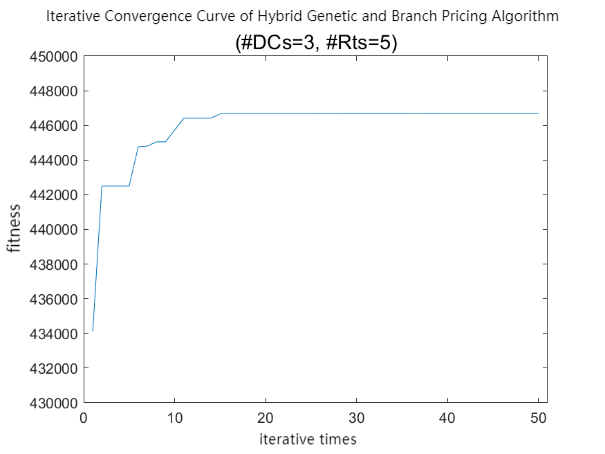
\includegraphics[width=\linewidth]{5-1}
        \label{fig:5-1}  
    \end{subfigure}
    \hfill
    \begin{subfigure}{0.45\textwidth}
        \centering
        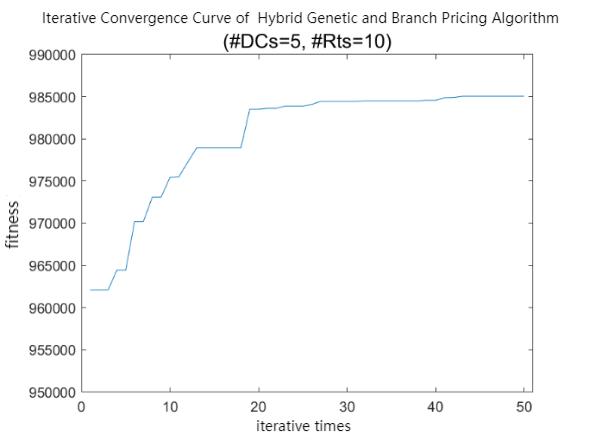
\includegraphics[width=\linewidth]{5-2}
        \label{fig:5-2}  
    \end{subfigure}
    \caption{Convergence behavior of the proposed algorithm across different problem scales}
    \label{fig:5-1&2}
\end{figure}
    
    From the experimental results of the two test cases, under a limited number of iterations, the hybrid genetic with branch-and-price algorithms converge at the 15th iteration for \#DCs=3, \#Rts=5, with a corresponding maximum fitness value of 446,665. For \#DCs=5, \#Rts=10, the hybrid genetic with branch-and-price algorithms converge at the 27th iteration, with a maximum fitness value of 984,450. Additionally, the hybrid genetic algorithm quickly achieves a good solution in the early iterations, with the maximum fitness of the model gradually increasing as the number of iterations grows, ultimately converging to a near-optimal value. The convergence speed, an important performance metric for genetic algorithms, indicates the number of iterations required to find the optimal solution. Generally, the faster the convergence speed, the better the performance of the genetic algorithm. Therefore, the hybrid genetic algorithm demonstrates good performance in solving medium- to small-scale problems.
    
    From the perspective of solution quality analysis, when solving the fitness value of each individual, precise solutions can be achieved under known conditions. Moreover, the optimal solution is always obtained at the root node of the branch-and-bound tree, meaning that the optimal solution obtained by solving the linear relaxation problem of the set covering model is an integer solution.
    \begin{itemize}
    \item \textbf{Comparing with the scenario without emission reduction technology investment}
    \end{itemize}
    
    Comparing the model with the scenario without emission reduction technology investment (setting $w_j=0$), Table \ref{tab:5-2} is obtained. It can be observed that when considering emission reduction technology investment, as the problem scale increases, the total profit of the enterprise continues to rise, while carbon emissions also increase. When the number of retailers is the same, a greater number of candidate distribution centers allows the enterprise to select more suitable distribution centers to serve retailers, thereby increasing total profit. Changes in carbon emissions depend on the enterprise's decisions. Furthermore, under the same problem scale, compared to no emission reduction investment, enterprises implementing emission reduction technology investment can achieve higher total profits while simultaneously reducing carbon emissions. This demonstrates the importance of investing in such emission reduction technologies for enterprises, as it not only increases profits but also enhances the enterprise's green development image.
    
    
    \begin{table}[htbp]
    \centering
    \caption{Comparison of results with and without emission reduction technology investment}
    \label{tab:5-2}
    \begin{tabular}{@{}ccccccccc@{}}
    \toprule
    \multirow{2}{*}{\#DCs} & \multirow{2}{*}{\#Rts} & \multicolumn{2}{c}{With Investment} & \multicolumn{2}{c}{Without Investment} & \multirow{2}{*}{Profit Increase} & \multirow{2}{*}{Emission Reduction} \\
    \cmidrule(lr){3-4} \cmidrule(lr){5-6}
     & & Profit & Emissions & Profit & Emissions & & \\
    \midrule
    3 & 5 & 458187.2 & 65048.5 & 442819 & 80856 & +3.47\% & -19.55\% \\
    3 & 10 & 745169 & 113038 & 703249.4 & 151335.2 & +5.96\% & -25.32\% \\
    5 & 10 & 885151 & 119775.2 & 854799.6 & 151916.6 & +3.55\% & -21.16\% \\
    5 & 20 & 1676735 & 199892 & 1535646 & 298334.2 & +9.18\% & -33.00\% \\
    5 & 30 & 2250450 & 259172 & 2175306 & 425793.2 & +3.45\% & -39.13\% \\
    \midrule
    \multicolumn{6}{c}{\textbf{Average}} & \textbf{+5.12\%} & \textbf{-27.63\%} \\
    \bottomrule
    \end{tabular}
    \end{table}
    
    
    \begin{itemize}
    \item \textbf{Impact of Changes in the Carbon Reduction Investment Cost Coefficient}
    \end{itemize}
    
    In this experiment, we adjust the $\delta$ value within $\theta_j(D_j)$ to observe how changes in the carbon reduction investment cost coefficient influence the firm’s decisions on location, pricing, reduction rate, as well as the effects on $D_j$, carbon reduction investment costs, total profits, and carbon emissions. The experiment uses 20 sets of instances with \#DCs = 3 and \#Rts = 10.  Each instance is run 10 times, with the results averaged over the 10 runs. Subsequently, the results for all 20 sets of instances are averaged, with final values rounded to one decimal place. The specific results are presented in Table \ref{tab:5-3} and Figure \ref{fig:5-3}.
    
    
    \begin{table}[htbp]
    \centering
    \caption{Experimental results with different $\delta$ values}
    \label{tab:5-3}
    \scriptsize
    \begin{tabular}{@{}l*{14}{r}@{}}
    \toprule
    \multirow{2}{*}{$\delta$} & 
    \multirow{2}{*}{\shortstack{Total\\Profit}} & 
    \multirow{2}{*}{\shortstack{Carbon\\Emission}} & 
    \multirow{2}{*}{\shortstack{Investment\\Cost}} & 
    \multirow{2}{*}{\shortstack{\#DCs\\Open}} & 
    \multirow{2}{*}{\shortstack{\#Rts\\Served}} & 
    \multicolumn{3}{c}{Emission Reduction} & 
    \multicolumn{3}{c}{Pricing} & 
    \multicolumn{3}{c}{Demand Served} \\
    \cmidrule(lr){7-9} \cmidrule(lr){10-12} \cmidrule(lr){13-15}
     & & & & & & $w_0$ & $w_1$ & $w_2$ & $p_0$ & $p_1$ & $p_2$ & $D_0$ & $D_1$ & $D_2$ \\
    \midrule
    1000 & 909350 & 5752 & 119126 & 2.6 & 10.0 & 0.964 & 0.866 & 0.987 & 60.4 & 67.0 & 70.2 & 9930 & 4300 & 12940 \\
    3000 & 775961 & 86269 & 81925 & 2.6 & 10.0 & 0.317 & 0.287 & 0.674 & 60.4 & 67.0 & 70.2 & 9930 & 4300 & 12940 \\
    5000 & 745169 & 113038 & 46304 & 2.4 & 9.6 & 0.183 & 0.189 & 0.424 & 60.4 & 67.0 & 70.2 & 9930 & 4300 & 12940 \\
    7000 & 732169 & 126223 & 32910 & 2.4 & 9.6 & 0.134 & 0.112 & 0.283 & 60.4 & 67.0 & 70.2 & 9930 & 4300 & 12940 \\
    9000 & 725538 & 132926 & 26123 & 2.4 & 9.6 & 0.127 & 0.085 & 0.255 & 60.4 & 67.0 & 70.2 & 9930 & 4300 & 12940 \\
    11000 & 721127 & 138666 & 19042 & 2.4 & 9.6 & 0.079 & 0.125 & 0.183 & 60.4 & 67.0 & 70.2 & 9930 & 4300 & 12940 \\
    13000 & 718457 & 135712 & 16074 & 2.4 & 9.4 & 0.071 & 0.064 & 0.124 & 60.4 & 67.0 & 70.2 & 9930 & 4300 & 10040 \\
    15000 & 715967 & 137453 & 15077 & 2.4 & 9.4 & 0.064 & 0.041 & 0.125 & 60.4 & 67.0 & 70.2 & 9930 & 4300 & 10040 \\
    17000 & 713753 & 139140 & 13177 & 2.4 & 9.4 & 0.042 & 0.063 & 0.125 & 60.4 & 67.0 & 70.2 & 9930 & 4300 & 10040 \\
    \bottomrule
    \end{tabular}
    \end{table}

In Table \ref{tab:5-3}, the average number of distribution centers opened decreases as the value of $\delta$ increases, indicating that changes in $\delta$ affect the enterprise's location decisions. The decision on the emission reduction rate $w_j$ by the distribution centers generally decreases as the value of $\delta$ increases. Specifically, when the value of $\delta$ is small, the optimal emission reduction rate for each open distribution center tends to be close to 1, resulting in high emission reduction technology investment costs. However, when the value of $\delta$ is large, the optimal emission reduction rate tends to approach or even reach 0, leading to lower emission reduction technology investment costs.     

From Figure \ref{fig:5-3}, it can be seen that as the value of $\delta$ increases, the total profit of the enterprise initially decreases and then stabilizes, eventually approaching the average total profit of 703,249.4 when emission reduction technology investment is not implemented. At the same time, carbon emissions initially rise and then gradually stabilize. Under the premise that the initial carbon emission quota remains unchanged, changes in the enterprise's carbon emissions will affect its carbon trading decisions. 


\begin{figure}[H]
    \centering
    \begin{tikzpicture}
    \begin{axis}[
        width=0.8\textwidth,
        height=0.6\textwidth,
        xlabel={$\delta$ value},
        ylabel={Total Profit (USD)},
        ylabel style={blue},
        ymin=700000, ymax=950000,
        xtick={1000,3000,5000,7000,9000,11000,13000,15000,17000},
        grid=major,
        legend pos=north west,
    ]
    
    \addplot[blue, mark=*, thick] coordinates {
        (1000, 909349.6)
        (3000, 775960.8)
        (5000, 745169.0)
        (7000, 732168.6)
        (9000, 725537.6)
        (11000, 721126.8)
        (13000, 718457.0)
        (15000, 715967.4)
        (17000, 713753.0)
    };
    \addlegendentry{Total Profit}
    \end{axis}
    \begin{axis}[
        width=0.8\textwidth,
        height=0.6\textwidth,
        axis y line=right,
        axis x line=none,
        ylabel={Carbon Emissions (kg $CO_2$)},
        ylabel style={red},
        ymin=5000, ymax=150000,
        grid=none,
        legend pos=north east,
    ]
    \addplot[red, mark=square*, thick] coordinates {
        (1000, 5751.7)
        (3000, 86268.9)
        (5000, 113038.0)
        (7000, 126223.4)
        (9000, 132926.0)
        (11000, 138665.6)
        (13000, 135712.2)
        (15000, 137453.0)
        (17000, 139140.4)
    };
    \addlegendentry{Carbon Emissions}
    \end{axis}
    \end{tikzpicture}
    \caption{Comparison of total profit and carbon emissions variation with $\delta$ value}
    \label{fig:5-3}
    \end{figure}


Additionally, changes in the value of $\delta$ also affect the total demand $D_j$ of retailers served by the distribution centers. A particularly noteworthy finding from Table \ref{tab:5-3} is the structural change in the supply chain network when $\delta$ exceeds 13,000. At this threshold, the average number of retailers served decreases from 10.0 to 9.4, with a significant reduction in demand served at one distribution center ($D_2$ drops from 12,940 to 10,040). This indicates that when emission reduction technology becomes prohibitively expensive ($\delta \geq 13,000$), the firm strategically contracts its network—opening fewer distribution centers (average 2.4) and serving fewer retailers, particularly abandoning some high-demand retailers. This finding reveals that excessively high emission reduction technology costs can fundamentally alter the scale and scope of the supply chain network, potentially triggering strategic contraction. Such contraction not only affects carbon emissions but also reshapes the firm's market coverage and competitive position.

In summary, changes in the emission reduction investment cost coefficient $\delta$ can influence location, inventory, pricing, carbon trading, and emission reduction technology investment decisions in supply chain network design. Furthermore, when $\delta$ reaches a certain threshold (approximately 13,000 in our experiments), the enterprise's total profit, carbon emissions, and optimal emission reduction rate all stabilize, approaching the state without emission reduction investment. Clearly, when $\delta$ is small, enterprises are more inclined to invest in emission reduction, especially when facing multiple investment options. They will prioritize emission reduction technologies corresponding to smaller $\delta$ values, allowing them to achieve better emission reduction results at lower costs and maximize profits. However, when the value of $\delta$ is sufficiently large, investing in emission reduction technology may no longer be a wise choice for the enterprise, and may even lead to strategic retrenchment in market coverage.


    
    
\section{Conclusion}

The escalating urgency of climate change has prompted governments worldwide to implement carbon emission policies, with cap-and-trade emerging as a pivotal market-based mechanism. For enterprises whose supply chains are major carbon emitters, navigating this regulatory landscape while maintaining profitability requires integrated strategic planning. This study addressed this challenge by developing a comprehensive Cap-and-Trade Supply Chain Network Design (CAT-SCND) model that jointly optimizes facility location, inventory management, pricing, carbon trading, and emission reduction technology investment—decisions traditionally studied in isolation.
Building upon these computational results, we consolidate the following key insights for managers.

\subsection{Summary of Findings and Managerial Insights}

Our study develops and solves an integrated Cap-and-Trade Supply Chain Network Design (CAT-SCND) model, yielding several key findings with direct managerial relevance:
\begin{enumerate}[label=(\arabic*), leftmargin=*]
    \item \textbf{The Win-Win Potential is Contingent on Technology Cost:} Strategic investment in emission reduction technology under cap-and-trade can create a win-win outcome, as evidenced by an average profit increase of \textbf{5.12\%} coupled with an average emission reduction of \textbf{27.63\%}. However, this potential is critically dependent on the technology's cost-effectiveness ($\delta$). The decision is not a simple yes/no but a matter of finding the optimal investment level $w_j^*$ that balances carbon savings against quadratic investment costs.
    \item \textbf{The Investment Cost Coefficient ($\delta$) is a Strategic Filter:} The parameter $\delta$ acts as a decisive filter for technology selection. A low $\delta$ justifies aggressive investment ($w_j \rightarrow 1$), transforming carbon allowances into a revenue stream. As $\delta$ increases, the optimal investment rate declines sharply. Beyond a critical threshold (approximately $\delta > 13,000$ in our setting), investment becomes minimal, and firms' operations converge to a non-investment baseline. This underscores the need for meticulous cost-benefit analysis in green technology procurement.
    \item \textbf{High Compliance Costs Can Trigger Network Reshaping:} Notably, when $\delta$ becomes prohibitively high, the model reveals a strategic contraction: firms may open fewer distribution centers and serve fewer retailers, even sacrificing some high-demand segments (as shown by the drop in $D_2$ in Table \ref{tab:5-3}). This highlights a previously under-explored risk—carbon constraints coupled with expensive abatement options can lead to a reduction in market coverage, not just operational tweaks.
    \item \textbf{Decisions are Deeply Intertwined:} The model confirms the necessity of an integrated optimization approach. The optimal emission reduction rate for a facility depends on the demand it serves, which in turn is determined by location and pricing decisions. Siloed decision-making is likely to yield suboptimal outcomes under the complex incentives created by cap-and-trade.
\end{enumerate}

\subsection{Theoretical Contributions and Future Research}
This study contributes to the literature on sustainable supply chain management by providing the first integrated optimization framework that simultaneously addresses location, inventory, pricing, carbon trading, and emission reduction technology investment under cap-and-trade policy. The proposed hybrid genetic algorithm with branch-and-price offers a viable solution methodology for this class of complex problems.

Several avenues for future research remain. First, extending the model to a multi-product setting would capture demand correlations and shared resources. Second, incorporating stochastic carbon prices and demand would enhance the model's realism. Third, considering capacity constraints for distribution centers and exploring dynamic, multi-period investment strategies are important directions. Finally, developing more scalable heuristics or decomposition techniques is essential for solving large-scale industrial instances.

    \bibliographystyle{plainnat}
    \bibliography{refs}
    
    \end{document}
    
    
    